\documentclass[10pt,a4paper]{article}
\usepackage[T1]{fontenc}
\usepackage[utf8]{inputenc}
\usepackage{lmodern,microtype,amsmath}
\usepackage[margin=18mm,top=18mm,bottom=19mm]{geometry}
\usepackage{graphicx,booktabs,tabularx,array,xcolor,fancyhdr,titlesec,fancyvrb}
\usepackage{tikz}
\usepackage{xurl}
\usepackage[colorlinks=true,urlcolor=teal,linkcolor=teal,hypertexnames=false]{hyperref}
\definecolor{forest}{HTML}{173C33}
\definecolor{muted}{HTML}{53665C}
\hypersetup{pdftitle={EcoSentinel: project report},pdfauthor={Mario Rodrigo, Sambhav and Wassim}}
\setlength{\parindent}{0pt}
\setlength{\parskip}{6pt}
\setlength{\emergencystretch}{3em}
\renewcommand{\arraystretch}{1.16}
\newcolumntype{Y}{>{\raggedright\arraybackslash}X}
\titleformat{\section}{\Large\bfseries\color{forest}}{}{0pt}{}
\titleformat{\subsection}{\normalsize\bfseries\color{forest}}{}{0pt}{}
\titlespacing*{\section}{0pt}{0pt}{9pt}
\titlespacing*{\subsection}{0pt}{8pt}{3pt}
\pagestyle{fancy}\fancyhf{}
\fancyfoot[L]{\footnotesize\color{muted}EcoSentinel / ADSDB P1}
\fancyfoot[R]{\footnotesize\thepage}
\renewcommand{\headrulewidth}{0pt}
\fvset{fontsize=\small,baselinestretch=1,listparameters={\setlength{\topsep}{4pt}\setlength{\partopsep}{0pt}}}
\newcommand{\refguide}[1]{\vfill{\footnotesize\color{muted}Further detail: #1\par}}
\begin{document}
\fontsize{10.5}{13.2}\selectfont
\thispagestyle{empty}
\section*{User manual / 1 of 2}
\textbf{Repository:} \url{https://github.com/SambhavMayani/ADSBDB}\\
\textbf{Authors:} Mario Rodrigo, Sambhav and Wassim.

These instructions use \textbf{Windows and Git Bash}, from the repository folder. Install 64-bit Python 3.11, Git and Docker Desktop first, then start Docker Desktop. You need Internet to install libraries and download models. Inference runs on CPU. No GPU or paid AI API is required. Linux instructions are in \path{README.md}.

\subsection*{1. Install the application and check the code}
\begin{Verbatim}
git clone https://github.com/SambhavMayani/ADSBDB.git
cd ADSBDB
python -m venv .venv
source .venv/Scripts/activate
python -m pip install -r requirements.txt
python -m pip check
python -m pytest -q
python -m orchestration.pipeline --plan
\end{Verbatim}
The tests should pass. The plan lists 16 steps without running them. Neither command needs your wildlife data or model weights. In each new terminal, return to this folder and activate \texttt{.venv} again. If the repository is private, the assessor needs access.

\subsection*{2. Download the pretrained models once}
Libraries contain the code. \textbf{Model weights} are the learned parameters that the code loads to process an image, sound or text. Downloading them does not train a model or create dataset embeddings. Prepare the embedding models \textbf{before running the pipeline}:
\begin{Verbatim}
python -m exploitation_zone.prepare_models --download
\end{Verbatim}
Expect \texttt{Embedding models ready}. For \textbf{Task 3 only}, also prepare Qwen and BLIP:
\begin{Verbatim}[fontsize=\footnotesize]
python -m multimodal_tasks.rag_model --download
HF_HUB_OFFLINE=0 python -c "from huggingface_hub import snapshot_download; \
from multimodal_tasks.generate import MODEL, REVISION; \
snapshot_download(repo_id=MODEL, revision=REVISION, token=False)"
\end{Verbatim}
Later runs reuse the local cache. The pipeline loads weights offline. Its acquisition option downloads \emph{wildlife data}, not models. Task 3 checks for 2.5 GiB of available RAM before generation. This is a guard, not a full machine specification. Close other applications if needed and allow minutes for CPU responses. Keep free disk space for weights, data and the query copy.

\subsection*{3. Start local object storage}
\begin{Verbatim}
cp -n .env.example .env
# Edit .env: set your local storage username and password.
docker compose up -d
python orchestration/check_minio_connection.py
\end{Verbatim}
Set \texttt{MINIO\_ROOT\_USER} and \texttt{MINIO\_ROOT\_PASSWORD} before creating a new storage service. Keep existing credentials when using a prepared installation. Never commit \texttt{.env}. Port 9000 is the S3 API and port 9001 is the storage console. The EcoSentinel interface uses a different port, shown on the next page.

\clearpage\thispagestyle{empty}
\section*{User manual / 2 of 2}
\subsection*{4. Choose the route that matches your data}
\textbf{A. Starting without local raw data.} Set the provider credentials in \texttt{.env}, including \texttt{XENO\_CANTO\_API\_KEY}, and review the species/acquisition settings in \texttt{config/}. Then run:
\begin{Verbatim}
python -m orchestration.pipeline --run --with-acquisition
\end{Verbatim}
This runs three download scripts and then the normal pipeline: 19 steps in total. Providers can change content or impose quotas. The default audio request is four recordings per species; shortages can stop acquisition. Inspect the log and keep successful downloads. If you decide to use the available smaller dataset, review its metadata and continue with route B. A fresh download need not reproduce our reference counts.

\textbf{B. Raw data already supplied locally.} Place the files and their matching \texttt{\_metadata.json} records under \path{data/raw_dataset/<modality>/<species_id>/}. Use the supplied/acquisition layout, since arbitrary files without provenance are insufficient. Run:
\begin{Verbatim}
python -m orchestration.pipeline --run
\end{Verbatim}
Expect \texttt{Pipeline status: completed}. The last step checks that accepted files and vector segments agree. Logs and the run JSON are under \path{reports/orchestration/}.

\textbf{C. Storage and Chroma already prepared.} Keep their matching data and model cache. Skip rebuilding and run \texttt{python -m orchestration.reconcile}. Expect \texttt{completed} and an empty \texttt{problems} list. Only the unchanged reference installation should have 198 accepted files and 6,021 vectors. Git contains neither that dataset nor the weights.

\subsection*{5. Prepare searches and open the interface}
Stop pipeline/index writers first. Use a \textbf{new, nonexistent destination}:
\begin{Verbatim}
python -m orchestration.audit --source data/chromadb \
  --snapshot data/search_index
python -m multimodal_tasks.search --status
python -m webapp.server
\end{Verbatim}
The first command verifies and copies the existing database. It does \textbf{not} run encoders again or copy media. Chroma already persists vectors on disk, but opening it can cause internal writes. Our interface therefore opens this separate copy to protect the original. The copy costs extra disk space and does not update itself. Reuse it while the data is unchanged. After an index update, create a new copy and pass its path with \texttt{-{}-index NEW\_PATH} to the search/web commands.

Open \textbf{http://127.0.0.1:8765}. The pipeline does not start the web automatically. Try an image in \emph{Buscar similares} for Task 1, a wildlife phrase in \emph{Explorar por texto} with mixed results for Task 2, and a habitat/diet question in the RAG tab for Task 3. Check the sources. Search quantity defaults to eight files and can be set to 1--50; CLI searches use \texttt{-{}-limit N}. Stop the server with Ctrl+C.

\subsection*{6. Inspect what the run produced}
Open \path{reports/trusted_quality/<modality>/<timestamp>/quality_report.html}. Keep its PNG files beside it. The same folder contains JSON summaries and CSV measurements. Expected results and recovery steps for all routes are in \path{docs/user_guide.md}. A run that fails a check needs investigation before its results can be accepted.

\clearpage\thispagestyle{empty}
\vspace*{22mm}
{\color{forest}\fontsize{40}{44}\selectfont\bfseries EcoSentinel\par}
\vspace{7mm}
{\LARGE Wildlife data, search and evidence\par}
\vspace{15mm}
{\large ADSDB P1\\Universitat Polit\`ecnica de Catalunya\par}
\vspace{13mm}
{\Large Mario Rodrigo\\Sambhav\\Wassim\par}
\vspace{8mm}29 October 2026
\vspace{16mm}
\subsection*{About this project}
EcoSentinel brings wildlife photographs, recordings and descriptions into one local system. We preserve the original files, check their quality and make them searchable. Users can find related material and ask questions whose answers point back to retrieved sources.

This report explains what we built and why. It separates the properties we have tested from the questions that still need a larger evaluation. The user manual comes first so that a new reader can install the application and inspect the work.

\vfill
\begin{tabularx}{\linewidth}{@{}Y r@{}}
Purpose, data and architecture & 1\\
Landing and Formatted & 2\\
Trusted decisions and quality reports & 3\\
Exploitation and model choices & 4\\
Similarity search and its limits & 5\\
Tasks 1 and 2, query preparation and interface & 6\\
Task 3: answers from retrieved evidence & 7\\
Orchestration, validation and reproducibility & 8
\end{tabularx}

\clearpage\setcounter{page}{1}
\section*{1. Purpose, data and architecture}
\subsection*{Why wildlife data?}
A photograph can show an animal, but it cannot tell the whole story. A field team may also need its call or a source that describes its habitat. These materials often sit in separate catalogues. We chose Iberian fauna to explore how one system could connect them within a clear, limited domain.

EcoSentinel could help teachers prepare wildlife lessons or help analysts review material related to an observation. A user can start with a file or a phrase, find related records and follow an answer back to its source. The intended value is less manual searching across catalogues. We have not measured time savings or tested a commercial service. Reliable species identification would also require expert evaluation.

\subsection*{What the reference dataset contains}
\begin{tabularx}{\linewidth}{@{}l r Y@{}}\toprule
\textbf{Type} & \textbf{Files} & \textbf{Sources}\\\midrule
Images & 100 & Wikimedia Commons: ten images per species\\
Audio & 34 & Xeno-canto: recordings for nine species\\
Text & 64 & 20 Wikipedia articles and 44 GBIF descriptions\\\bottomrule
\end{tabularx}

The ten species include the Iberian lynx, wolf, deer, wild boar, eagle, eagle owl, kingfisher, robin, Perez's frog and ocellated lizard. Scientific identifiers in \path{config/species.yaml} link records across zones. Audio adds a useful ecological view, but coverage is uneven: the lizard has no recording and the lynx has only two. Text also varies by species and source. We keep these gaps visible instead of treating the sample as representative of Iberian biodiversity.

The acquisition scripts save URLs, provider identifiers and available licence/attribution fields beside each raw file. Wikipedia records also retain revision information. Provider labels help trace the data; they are not expert checks of the species. Some audio licences restrict commercial reuse, so any future business use would need to review permissions for each asset.

\subsection*{Why four zones?}
\begin{center}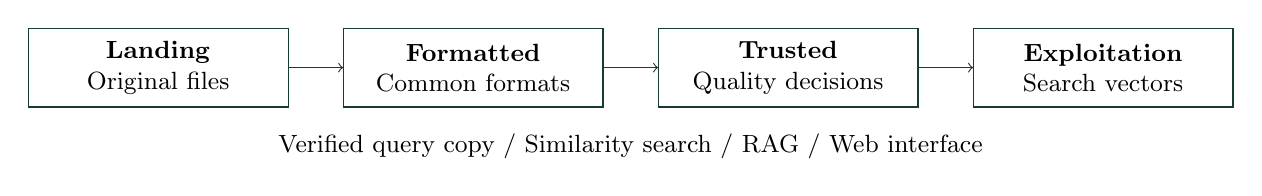
\begin{tikzpicture}[every node/.style={font=\small,align=center}]
\foreach \x/\a/\b in {0/Landing/Original files,4/Formatted/Common formats,8/Trusted/Quality decisions,12/Exploitation/Search vectors}{\node[draw=forest,minimum width=3.3cm,minimum height=1cm] at (\x,0) {\textbf{\a}\\\b};}
\foreach \x in {1.65,5.65,9.65}{\draw[->,forest] (\x,0)--(\x+0.7,0);}
\node at (6,-1) {Verified query copy / Similarity search / RAG / Web interface};
\end{tikzpicture}\end{center}
Each zone answers a different question: what arrived, how it is represented, whether it is usable, and how to search it. This separation lets us change a quality rule or encoder without losing the original evidence. Python packages follow these boundaries. S3 object storage suits the large, varied media files; separate buckets distinguish their processing state. Chroma stores vectors locally without requiring another database server. The Docker configuration pins the S3-compatible storage service.

We use one orchestrator to connect the stages, but keep their code independently testable. Models run sequentially on CPU to limit memory use. Acquisition remains optional, so supplied data can follow the same route without downloading it again.
\refguide{\path{docs/data_sources.md}, \path{docs/p1_requirements.md}.}

\clearpage
\section*{2. Landing and Formatted}
\subsection*{A cheap identity check before model processing}
Landing first checks input type, signatures, basic structure and resource limits. The Security Gate can block a disguised executable or an unsafe archive before expensive decoding. It is an input check, not an antivirus scanner. Accepted files enter Temporal Landing, then a verified copy goes to Persistent Landing, organised by modality and species.

The Temporal key combines \textbf{the first 16 hexadecimal characters of SHA-256 and the filename}. SHA-256 reads the bytes in small blocks. It needs neither media decoding nor model weights, so its cost is simpler and smaller in scope than neural inference. We did not benchmark a speed ratio. Hashes answer an identity/integrity question; embeddings answer a similarity question.

\begin{tabularx}{\linewidth}{@{}l l Y@{}}\toprule
\textbf{Bytes} & \textbf{Name} & \textbf{Landing result}\\\midrule
Same & Same & Reuse the existing, verified record\\
Same & Different & Ingest a separate submitted-file record\\
Different & Same & Ingest under a new hash; preserve the earlier file\\
Different & Different & Ingest a new record\\\bottomrule
\end{tabularx}

Keeping the filename preserves the identity of the submitted file, even when two names contain identical bytes. This can cost extra storage. Trusted performs the later content duplicate check. The shortened key hash is not collision-proof; copy verification uses the full SHA-256, metadata and byte length.

A completion record points to the Persistent copy. If the file has left Temporal, ingestion checks this record and the target before skipping it. A missing target or conflicting species/source is an error. We write completion only after verifying the copy and retain Temporal files by default. This ordering makes interrupted copies recoverable. The record confirms Landing completion, not acceptance in Trusted.

\subsection*{Formats chosen for photographs, calls and descriptions}
\textbf{Images become RGB JPEG at quality 95.} Wildlife photographs contain continuous colour and texture, for which JPEG usually needs less space than lossless PNG. Quality 95 is a conservative size/detail compromise, not a measured optimum. We preserve dimensions and EXIF orientation without rotating or cropping. White replaces transparency. JPEG still loses information, so the original remains available. MPO contains several photographs in one file, sometimes named \texttt{.jpg}. We use its first frame: six reference files produce six JPEGs, with eight extra frames preserved upstream.

\textbf{Audio becomes FLAC PCM16.} A faint animal call can overlap with rain, wind or other species. We avoid another lossy audio encoding step that could remove useful detail. FLAC compresses the resulting PCM samples losslessly and usually uses less space than uncompressed PCM. We keep rate, channels, background sound and quiet intervals. Converting richer sources to 16-bit can still reduce precision, and FLAC cannot recover detail already lost in an MP3. Encoder-specific resampling happens later.

\textbf{Text becomes UTF-8 with NFC characters and LF line endings.} This keeps Spanish and English consistent across source formats without removing case or punctuation. JSON extraction first looks for recognised content keys at the shallowest depth, with fixed tie priorities. Only then does it fall back to the longest non-empty string. Arrays are processed per record. We record the extraction method/path because this rule can miss the author's intended field. Original files preserve any lost structure.
\refguide{\path{docs/landing_zone_documentation.md}, \path{docs/formatted_zone_documentation.md}.}

\clearpage
\section*{3. Trusted decisions and quality reports}
Trusted checks usability and provenance before choosing a search model. Policies live in YAML so that the rules and their versions can be inspected. A technical failure can reject a file. A warning records uncertainty while keeping potentially useful material.

\begin{tabularx}{\linewidth}{@{}p{.14\linewidth}Y Y@{}}\toprule
\textbf{Type} & \textbf{Checks and decisions} & \textbf{Reason}\\\midrule
Images & Decode; provenance; 20 MB, 40 MP and at least 128 pixels per side. Exact hashes, then pHash candidates checked with structure/colour. & Compressed size alone cannot bound decoding memory. Very small images have little usable detail. Duplicate confirmation is stricter than a perceptual hash alone.\\
Audio & Decode; provenance; 200 MB cap; duration and amplitude measurements; exact PCM duplicates. & Recordings can be longer than image files. Quiet or distant calls may still be useful, so low energy produces a warning.\\
Text & Strict decoding; provenance; 4 MB cap; exact duplicates, near-duplicate warnings and privacy-pattern counts. & Species descriptions should remain manageable. Short GBIF records and long articles need different interpretation, not an arbitrary common length.\\\bottomrule
\end{tabularx}

These byte limits use decimal MB. They are operational budgets for this local prototype, not biological boundaries or values proven optimal by experiments. Pixel limits complement byte limits. Audio memory also depends on duration and decoding, so its byte cap cannot guarantee a fixed RAM peak. The policies can be revised with measurements on a larger dataset.

Darkness, low sharpness, monochrome appearance and possible watermarks generally remain warnings. We do not crop, denoise or remove quiet audio sections: those actions could change the ecological evidence. A later failure or rejection keeps previously accepted bytes and records the changed status. Reconciliation then exposes outdated index references instead of silently deleting data.

\subsection*{Reports explain the decision for each file}
Each check produces JSON under \path{trusted-zone/_quality/<modality>/}, including the source, policy, decision, reasons and measurements. Report generators aggregate the current stored records, including earlier runs. They do not decode every file again or change acceptance decisions.

The local output includes an \textbf{HTML report}, a \textbf{JSON summary}, a \textbf{CSV table} and \textbf{PNG charts}. Images record dimensions, megapixels, size, brightness, sharpness and aspect ratio. Audio records duration, sample rate, channels, RMS/peak level, clipping and low-energy frames. Text records characters, words, vocabulary ratios and privacy-pattern counts without publishing the matched private values. Statistics and plots expose long files, quality warnings and uneven coverage. Before/after species distributions and source-field completeness help show whether filtering changed the collection.

\subsection*{What the reference reports show}
All 198 reference files remain accepted. The image report flags 32 possible watermarks and 14 monochrome-like images; these are heuristic flags, not confirmed defects. Audio has nine low-energy and two low-RMS flags. Its median duration is 40.91 seconds and its longest recording is 752.37 seconds. Text has a median of 208.5 words, ranging from 33 to 13,869. Source-field completeness is 100\%, but populated fields do not prove correct labels. Species distributions remain unchanged, including the missing lizard audio.

These results describe a curated batch. Synthetic malformed files and fault tests exercise rejection separately. We still need labelled examples to measure watermark and duplicate-detection accuracy. Pairwise text comparison will also need a more efficient candidate index as the dataset grows.
\refguide{\path{docs/trusted_zone_documentation.md}; reference summaries in \path{docs/evidence/quality_*.json}.}

\clearpage
\section*{4. Exploitation and model choices}
An embedding is a list of numbers that a model uses to represent content. Similar meanings can produce nearby vectors, even when file bytes differ. Exploitation creates these vectors from accepted Trusted files and stores them in five Chroma collections.

\begin{tabularx}{\linewidth}{@{}Y l r r@{}}\toprule
\textbf{Collection} & \textbf{Model family} & \textbf{Dimensions} & \textbf{Vectors}\\\midrule
Images & CLIP & 512 & 100\\
Audio & CLAP & 512 & 357\\
Text & Multilingual E5 & 384 & 547\\
Image and text & CLIP-aligned & 512 & 1,763\\
Audio and text & CLAP & 512 & 3,254\\\midrule
Total & & & 6,021\\\bottomrule
\end{tabularx}

\subsection*{Why these models?}
\textbf{CLIP} was trained to relate images and text. It supports both visual similarity and text-to-image retrieval. Our configured multilingual text adapter uses the compatible CLIP image space, which helps with Spanish and English queries. \textbf{CLAP} provides an aligned audio/text space, allowing a description of an animal sound to retrieve recordings. \textbf{Multilingual E5} handles text-to-text retrieval with its required \texttt{query:} and \texttt{passage:} prefixes. Its small variant limits CPU and memory costs.

One encoder would simplify the software but would not provide all these trained relationships. We selected models that match each task and can run locally. Their suitability for this prototype does not establish that they are the best models for Iberian fauna. That claim would require labelled retrieval comparisons. Model identifiers and pinned revisions are recorded in the configuration and provenance documentation.

\subsection*{Why 6,021 vectors for only 198 files?}
Long inputs need smaller parts because encoders have limited input lengths. E5 uses text chunks of 320 tokens with 40-token overlap. The image/text route uses 96 with 12-token overlap, and the audio/text route uses 60 with eight-token overlap. These budgets suit their configured text encoders. Overlap reduces the risk of splitting a useful sentence at a boundary, at the cost of extra vectors.

Audio uses ten-second windows after encoder preparation to 48 kHz mono. A window keeps a local call searchable instead of averaging a long recording into one vector. This step belongs to the model, so Trusted can retain the original rate and channels for other uses. Text also appears in shared collections, which explains much of the extra vector count. Results later group segments back into files.

\subsection*{Persistent, incremental indexing}
Vectors remain on disk in \path{data/chromadb/}. Metadata links each part to its source file, model/policy version and position. An unchanged file with all expected parts is skipped on a rerun. Source checksums, policy fingerprints and complete part sets determine reuse; a matching total count alone is insufficient. Interrupted publication can be repaired by processing the incomplete asset again.

The indexer loads models sequentially on CPU and uses bounded batches. This reduces simultaneous memory use, although long audio still needs care during decoding. The application opens a verified query copy rather than the original database because Chroma may write internal state when opened. Copying stored vectors is inexpensive compared with computing them again, but takes disk space and must be repeated after updates. It protects the original index; it is not required to make vectors persistent.
\refguide{\path{docs/exploitation_zone_documentation.md}, \path{docs/data_sources.md}, \path{config/exploitation.yaml}.}

\clearpage
\section*{5. Similarity search and its limits}
\subsection*{Cosine measures direction in one vector space}
For two non-zero vectors, cosine similarity is
\[
  s(q,x)=\frac{q\cdot x}{\lVert q\rVert\lVert x\rVert}.
\]
We normalise both vectors, so this becomes a dot product. Values range from $-1$ to $1$, with larger values meaning closer directions. Chroma returns cosine distance; we display $1-\text{distance}$. We reject non-finite or incompatible vectors rather than returning misleading scores.

For an illustrative query $q=(1,0)$, the unit vectors $(0.96,0.28)$, $(0.6,0.8)$ and $(0,1)$ score 0.96, 0.60 and 0.00. The first is closest in this example. These numbers are not probabilities that two animals share a species. Real scores depend on the model and query type, so there is no universal ``correct match'' threshold in our interface.

\subsection*{Exact search for small sets; HNSW for larger sets}
The application counts \textbf{eligible vectors after filters}. With \textbf{64 or fewer}, it reads the vectors and compares every one. With \textbf{65 or more}, it asks Chroma's \textbf{HNSW} index. HNSW, or Hierarchical Navigable Small World, is a graph search method: it navigates from coarse graph levels to nearby candidates instead of comparing every vector. It is approximate, so it can miss an exact nearest neighbour.

Why choose 64? We wanted a small, bounded exact scan that also works for tiny or new Chroma segments without a persisted HNSW reader. At 512 dimensions, 64 dot products involve 32,768 vector components. The float32 vector payload alone is 128 KiB, excluding metadata, Python objects and normalisation work. This makes the scale of the fallback explicit. \textbf{We did not benchmark 32, 64 and 128 to find an optimum.} Another small cap could work; changing it should follow timing and recall measurements. Tests cover both 64 and 65, including filtered collections. The cap counts vector parts, not returned files and not vector dimensions.

For larger sets, we expand the retrieved candidate pool when many matches belong to one file. We then keep distinct assets, so a long recording cannot fill the result list merely because it has many segments. \textbf{Top-k} means the maximum number of returned files: default eight, selectable from 1 to 50 in the interface or with \texttt{-{}-limit N}. Filters or limited data can produce fewer results.

\subsection*{Different modalities need a shared trained space}
An image and a sentence can be compared when their encoders share a trained CLIP space. The same applies to CLAP audio and text. E5 lives in its own space. Even though CLIP and CLAP both produce 512 numbers, their coordinates mean different things. Computing their cosine would produce a number without a valid similarity interpretation, so we keep those collections separate.

When a query uses several spaces, \textbf{reciprocal rank fusion (RRF)} combines positions rather than raw cosine values. Each file receives $1/(60+r)$ from each ranking where it occurs at position $r$, counted once per ranking. The constant 60 smooths the advantage of the first few ranks; it is separate from top-k and has not been tuned on labelled wildlife queries. A visible modality allocation can then keep mixed results useful. This output is a combined ranking, not one global cosine ranking.

We therefore distinguish correct search mechanics from useful biological retrieval. Tests can verify filtering, grouping and score handling. Expert relevance labels are still needed to measure recall, ranking quality and species-related errors.
\refguide{\path{multimodal_tasks/search.py}, \path{docs/multimodal_tasks_documentation.md}.}

\clearpage
\section*{6. Tasks 1 and 2, queries and interface}
\subsection*{Task 1: find similar material of the same type}
A photograph retrieves photographs, a recording retrieves recordings, and text uses E5 to retrieve descriptions. For a stored record, we reuse its vector and exclude that entire file from the results, including its other segments. For an upload, we prepare the bytes in memory and use the same encoder and vector normalisation as the indexed data.

This supports questions such as ``Which stored photographs look like this one?'' A high-ranking image may share colour, pose or background without showing the same species. The result cards expose the source and score so that the user can inspect the candidates rather than accept a biological label automatically.

\subsection*{Task 2: search across types of material}
The image/text and audio/text collections each contain both types of data. A text phrase can retrieve photographs and descriptions through CLIP, or recordings and descriptions through CLAP. Image and audio queries can also retrieve mixed results in their compatible spaces. When searching all spaces, RRF combines the rankings as explained on page 5.

We group results by file and allocate available places across modalities. This helps a user see related evidence without a large number of text chunks taking every place. The trade-off is that the final order serves mixed exploration rather than pure cosine ranking. A heavily filtered search can still return only one modality.

\subsection*{Queries reuse processing without entering the dataset}
After the supervisor's clarification, we reuse Formatted conversions for external queries: RGB JPEG quality 95 for images, FLAC PCM16 for audio and canonical text. We then apply the same encoder preparation as during indexing. A stored Trusted JPEG bypasses another JPEG encode. Consistent processing reduces avoidable differences, but cannot undo previous compression damage or guarantee identical vectors for separately encoded files.

Shared Trusted measurements report blur, darkness, small image size or quiet audio as warnings. We deliberately omit duplicate rejection: a user may be looking for an existing image. We also avoid an uncalibrated watermark rule that could remove useful query information. Hard guards still reject invalid inputs, uploads above 10 MiB, images above 20 MP, and audio above 30 seconds or eight channels before conversion. These tighter query budgets keep interactive CPU work bounded; they are operational choices rather than accuracy thresholds.

Uploads stay in memory and are not added to MinIO or Chroma. The response includes an input hash and preparation details for traceability. Quality warnings are visible to the user and stay outside the RAG prompt because a blur measurement is not evidence about an animal.

\subsection*{A local interface for all three Tasks}
\begin{tabularx}{\linewidth}{@{}p{.34\linewidth}Y@{}}\toprule
\textbf{Tab} & \textbf{What the user can try}\\\midrule
Explorar por texto & A text query in E5, either shared space or all spaces; species filters and result quantity.\\
Buscar similares & An image or short recording; same-type or mixed retrieval, with related-file actions.\\
Preguntar al corpus / RAG & A question with an optional image; cited claims, candidate species, quality notes and response status.\\\bottomrule
\end{tabularx}

Here, ``corpus'' simply means the stored collection of documents and media. The static frontend needs no separate build tool. The Python server binds to the local machine, checks host/origin and serialises CPU requests. This makes classroom setup simpler. A public multiuser service would need authentication and a different deployment design.
\refguide{\path{docs/user_guide.md}, \path{docs/multimodal_tasks_documentation.md}.}

\clearpage
\section*{7. Task 3: answers from retrieved evidence}
Task 3 uses retrieval augmented generation, or \textbf{RAG}. The system first finds relevant stored information, then gives selected passages to a language model. This makes it possible to show where an answer came from and to decline a question when the evidence is insufficient.

\subsection*{How a question with an image is answered}
The uploaded image receives the shared preparation described on page 6. CLIP finds visual candidates and BLIP produces an automatic caption. Candidate species names guide searches for the requested subject, such as habitat or diet. E5 retrieves text, while a bounded lexical search helps find explicit words for those subjects. A global search remains available so that one visual candidate does not decide the whole answer.

The evidence selector keeps at most eight literal units and 1,600 characters for generation. These limits control prompt size and CPU cost. Full references remain available in the interface. The prompt tells the model to use the supplied evidence and keep uncertainty about the photographed animal. We avoid repeating a noisy caption in every biological search.

\textbf{Qwen receives text, not image pixels.} BLIP is the image-to-text step. Its caption can be wrong: in the recorded frog example it described ``a frog with a dumb barbell''. We treat this as a model observation, never as a verified identification. Similar frog references can still support a conditional answer about the retrieved candidates' habitat or diet.

\subsection*{Why Qwen and a separate captioning model?}
We use Qwen2.5-3B-Instruct in Q4\_K\_M GGUF form through llama.cpp. Quantisation reduces the model's memory needs, making CPU execution possible without a paid API. The model file is pinned and checked by SHA-256. BLIP gives us a separate image captioning step that we can inspect and test. This design loses some visual detail compared with a model that directly reads images, but keeps the components manageable on our machine. We have not established superiority over larger models or native visual assistants.

Generation uses a JSON grammar, then checks the response structure, allowed evidence IDs and exact quote matches. Multi-aspect questions can produce up to two claims. If one aspect has no support, it can remain empty and the interface reports a partial answer. These checks catch invented reference IDs and quotes. They do \textbf{not} prove that the model interpreted a passage correctly.

\subsection*{Failure handling and what we have validated}
An evidence-based abstention differs from invalid JSON, a timeout or an incomplete output. The interface keeps references visible and exposes the status. Generation has a 320-token output limit, a 120-second timeout, four CPU threads and a 2.5 GiB available-memory check. An inspectable vocabulary gate rejects unrelated questions before costly generation, but it can miss valid phrasing. Both this gate and the aspect rules need broader language evaluation.

Earlier native checks exercised text habitat, stored-image habitat, conditional frog identification, an unsupported genome question and an unrelated request. A separate frog habitat/diet browser run took 131.8 seconds overall, including 76.1 seconds of generation. One lynx answer was less directly relevant. These runs show that the system can execute the workflow; they are not an accuracy benchmark. The later query-preparation revision has offline regression tests, but those historical native runs were not repeated for it.

We therefore present candidate species and cited claims with their limits. A useful next evaluation would label external queries, compare retrieved passages and count both unsupported answers and unnecessary abstentions.
\refguide{\path{docs/generative_tasks_documentation.md}, \path{docs/evidence/native_models.json}. Model cards: \href{https://huggingface.co/Qwen/Qwen2.5-3B-Instruct-GGUF}{Qwen GGUF} and \href{https://huggingface.co/Salesforce/blip-image-captioning-base}{BLIP}.}

\clearpage
\section*{8. Orchestration, validation and reproducibility}
\subsection*{The 16 steps, in execution order}
\begin{tabularx}{\linewidth}{@{}l Y@{}}\toprule
\textbf{Stage} & \textbf{Numbered steps}\\\midrule
Storage & 1 Check connection; 2 create missing buckets\\
Landing & 3 Ingest local raw files; 4 copy and verify in Persistent\\
Formatted & 5 Format images; 6 format audio; 7 format text\\
Trusted & 8 Validate images; 9 validate audio; 10 validate text\\
Exploitation & 11 Index images; 12 text; 13 audio; 14 image/text; 15 audio/text\\
Verification & 16 Reconcile accepted files and vector parts\\\bottomrule
\end{tabularx}

The stages run sequentially. Optional acquisition adds three downloads after storage setup. Subprocesses use the active Python interpreter, with timeouts and UTF-8 logs. An atomic JSON report records progress. A failure stops later stages; restarting checks stored state and retries incomplete work. A local lock prevents two orchestrator runs in the same checkout. It does not coordinate other machines or manual writers, and there is no transaction across all zones.

\subsection*{Tests target behaviour and failure recovery}
The offline suite currently passes \textbf{469 tests}, with \textbf{72.37\% statement coverage} (29 October). It uses generated files, storage doubles, temporary real Chroma databases and local HTTP requests. Tests check conversion, metadata, duplicates, query limits, citations, idempotence and failure recovery. The latest additions test Landing completion records, conflicting sources, interrupted storage access, preserved outputs, rejected Trusted records and missing/stale vector parts. They also check the exact-search boundary at 64/65 eligible vectors.

Coverage records which measured statements ran. It neither measures model accuracy nor proves that every outcome was checked. We retain the same measurement scope. Some paths need separate storage or model checks; others remain untested. Meaningful assertions matter more than reaching 100\% by executing lines without checking results.

\begin{tabularx}{\linewidth}{@{}>{\raggedright\arraybackslash}p{.25\linewidth}Y@{}}\toprule
\textbf{Evidence} & \textbf{What it establishes}\\\midrule
Earlier isolated integration & One complete S3/Chroma test with deterministic encoders, including repeat execution.\\
Earlier CPU demonstration & Three synthetic assets produced seven vectors; the second run added zero. Native retrieval/RAG were checked separately.\\
Earlier preservation checks & Original Chroma file hashes/counts and S3 keys, sizes and ETags were compared without rebuilding the reference.\\\bottomrule
\end{tabularx}

\subsection*{Automatic checks and honest limits}
GitHub Actions runs the configured tests after pushes and pull requests. Fresh Windows/Linux jobs install the same requirements, check style and run offline tests with a 60\% coverage floor. A Linux job tests isolated S3 storage. The floor catches large regressions; it is not a quality score. Test reports remain available as job artifacts. Before submission, verify a green Actions run for the actual submitted commit. Local success cannot establish that result.

A clone reproduces the code tests and synthetic demonstration. Reproducing the 198-file reference also needs its data handoff, metadata and pinned model cache. New downloads can change. The query copy can become stale, long audio can use substantial RAM, and text duplicate comparisons are quadratic. We have no labelled retrieval or biological benchmark. These are explicit limits of the prototype, with tests and documentation that make its current guarantees reviewable.
\refguide{\path{docs/pipeline_orchestration.md}, \path{docs/testing_and_validation.md}, \path{docs/evidence/}.}
\end{document}
